%%%%%%%%%%%%%%%%%%%%%%%%%%%%%%%%%%%%%%%%%%%
%%%%%%%%%%%%%%%%%%%%%%%%%%%%%%%%%%%%%%%%%%%
%%%%%%%%%%%%%%% CHAPTER 12 %%%%%%%%%%%%%%%%


\section{Resposta em frequência}

\frame{
\frametitle{Introdução}
\begin{block}{Contextualização}
No regime permanente, \textbf{entradas senoidais} aplicadas a sistemas lineares geram \textbf{respostas senoidais} de mesma frequência.
\begin{itemize}
    \item Embora essas respostas tenham a mesma frequência das entradas, elas diferem em \textbf{amplitude e em fase}.
    \item Essas diferenças são \textbf{funções da frequência}.
\end{itemize}
\end{block}
}

\frame{
\frametitle{Introdução}
\begin{block}{Definição}
O termo \textbf{resposta em frequência} significa a resposta em regime permanente de um sistema a uma \textbf{entrada senoidal}. Nos métodos de resposta em frequência, variamos a frequência do sinal dentro de um certo intervalo e estudamos a resposta resultante.
\begin{itemize}
    \item Uma vantagem do método de resposta em frequência é que podemos utilizar os dados obtidos diretamente a partir das \textbf{medições} feitas nos sistemas físicos, sem a necessidade de recorrermos aos respectivos modelos matemáticos.
\end{itemize}
\end{block}
}

\frame{
\frametitle{Fasores}
\begin{block}{Introdução}
As senoides podem ser representadas por \textbf{números complexos} chamados \textbf{fasores}.
\begin{itemize}
    \item A resolução de circuitos de corrente alternada no domínio do tempo gera equações com soluções complexas e/ou trabalhosas. A análise destes circuitos por meio do uso de fasores e impedância proporciona uma maneira simplificada de resolvê-los.
\end{itemize}
\end{block}
}

\frame{
\frametitle{Fasores}
\begin{block}{Definição}
\begin{itemize}
    \item A \textbf{magnitude} do número complexo é a \textbf{amplitude} da senoide.
    \item O \textbf{ângulo} do número complexo é a \textbf{fase} da senoide.
\end{itemize}
\vspace{0.5cm}
Dada a senoide $x(t) = M_1 \ cos(\omega t + \phi_1)$, \\
    $$X = M_1 \phase{\phi_1} \ \text{é a representação fasorial da senoide} \ x(t)$$
\end{block}
}

\frame{
\frametitle{Fasores}
\begin{block}{O conceito da resposta em frequência}
O produto do fasor de entrada pela função do sistema resulta na representação do fator de saída.
\end{block}
\centerline{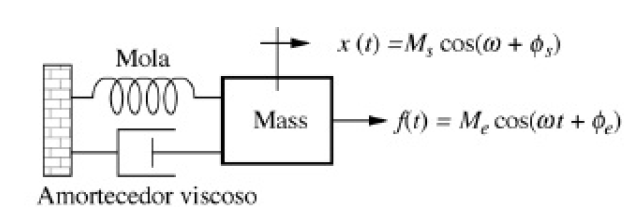
\includegraphics[width=0.7\linewidth]{Figuras/Ch12/fig1.PNG}}
}

\frame{
\frametitle{Fasores}
\begin{block}{O conceito da resposta em frequência}
Deste modo, a \textbf{saída do sistema} é dada por:
$$M_s(\omega) \phase{\phi_s}(\omega) = M_e(\omega) M(\omega) \phase{\phi_e (\omega) + \phi (\omega)}$$
\end{block}
\centerline{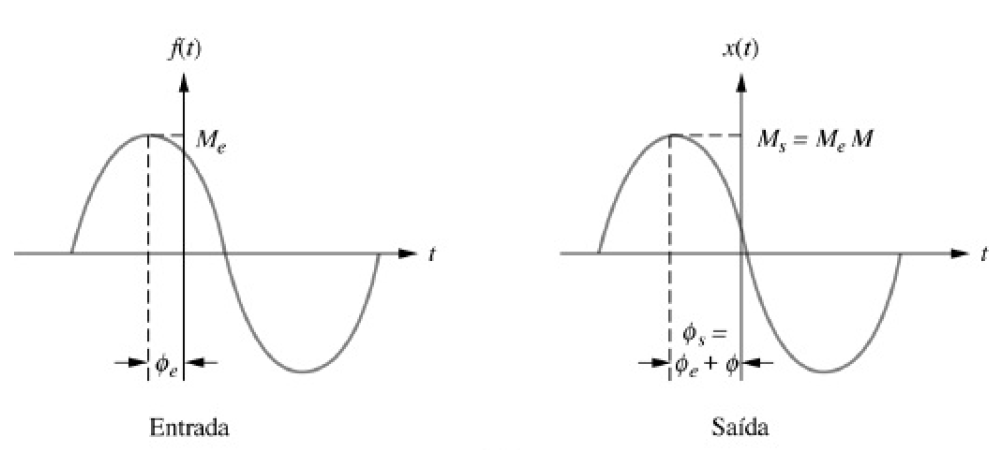
\includegraphics[width=1\linewidth]{Figuras/Ch12/fig2.PNG}}
}

\frame{
\frametitle{Fasores}
\begin{block}{O conceito da resposta em frequência}
A partir da equação anterior, observamos que a \textbf{função do sistema} é dada por:
$$M(\omega) = \dfrac{M_s(\omega)}{M_e(\omega)}$$
$$\phi (\omega) = \phi_s (\omega) - \phi_e (\omega)$$
\begin{itemize}
    \item $M(\omega)$: \textbf{magnitude} da resposta em frequência.
    \item $\phi (\omega)$: \textbf{fase} da resposta em frequência.
    \item $M(\omega) \phase{\phi}(\omega)$: \textbf{resposta em frequência}.
\end{itemize}
\end{block}
} 

\frame{
\frametitle{Resposta de regime permanente a uma entrada senoidal}
\begin{block}{Formulação matemática}
Considere um sistema de segunda ordem na forma:
$$M\ddot{x}(t) + B\dot{x}(t) + Kx(t) = F \ sen(\omega t)$$
Na forma padrão, podemos reescrever como sendo:
$$\ddot{x}(t) + 2\zeta\omega_n\dot{x}(t) + \omega_n^2x(t) = f \ sen(\omega t)$$
\begin{itemize}
    \item A \textbf{saída em regime permanente} será da forma:
\end{itemize}
$$x_p(t) = A \ sen(\omega t + \phi) = A_2 \ cos(\omega t) + A_1 \ sen(\omega t)$$
onde
$$A = \sqrt{A_1^2 + A_2^2}$$
$$\phi = \text{arctg}\Big(\dfrac{A_2}{A_1}\Big)$$
\end{block}
}

\frame{
\frametitle{Resposta de regime permanente a uma entrada senoidal}
\begin{block}{Formulação matemática}
\begin{itemize}
    \item $x_p(t) = A_2 \ cos(\omega t) + A_1 \ sen(\omega t)$
    \item $\dot{x}_p(t) = -\omega A_2 \ sen(\omega t) + \omega A_1 \ cos(\omega t)$
    \item $\ddot{x}_p(t) = -\omega^2[A_2 \ cos(\omega t) + A_1 \ sen(\omega t)]$
\end{itemize}
\vspace{0.5cm}
Substituindo $x_p(t)$, $\dot{x}_p(t)$ e $\ddot{x}_p(t)$ em $\ddot{x}(t) + 2\zeta\omega_n\dot{x}(t) + \omega_n^2x(t) = f \ sen(\omega t)$:
\begin{equation*}
\begin{split}
-\omega^2[A_2 \ cos(\omega t) + A_1 \ sen(\omega t)] + \\
+ 2\zeta\omega_n[-\omega A_2 \ sen(\omega t) + \omega A_1 \ cos(\omega t)] + \\
+ \omega_n^2 [ A_2 \ cos(\omega t) + A_1 \ sen(\omega t)] = \\
= f \ sen(\omega t)
\end{split}
\end{equation*}
\end{block}
}

\frame{
\frametitle{Resposta de regime permanente a uma entrada senoidal}
\begin{block}{Formulação matemática}
Rearranjando os termos, obtemos:
\begin{equation*}
\begin{split}
[-\omega^2A_2 + 2\zeta\omega_n \omega A_1 + \omega_n^2 A_2] \ cos(\omega t) + \\
+ [-\omega^2 A_1 - 2\zeta\omega_n \omega A_2 + \omega_n^2 A_1 - f]\ sen(\omega t) = 0
\end{split}
\end{equation*}
\begin{itemize}
    \item Fazendo $t = 2\pi/\omega$ e $t = \pi/2\omega$, obtemos: \\
\end{itemize}
\begin{equation*}
\begin{cases}
(\omega_n^2 - \omega^2)A_2 + 2\zeta\omega_n \omega A_1 = 0 \\
- 2\zeta\omega_n \omega A_2 + (\omega_n^2 - \omega^2)A_1 = f
\end{cases}
\end{equation*}
\begin{itemize}
    \item Multiplicando a primeira equação por $2\zeta\omega_n \omega$ e a segunda por $\omega_n^2 - \omega^2$, e somando as duas, chega-se em: \\
\end{itemize}
$$A_1 = \dfrac{(\omega_n^2 - \omega^2)f}{(2\zeta\omega_n \omega)^2 + (\omega_n^2 - \omega^2)^2}$$
\end{block}
}

\frame{
\frametitle{Resposta de regime permanente a uma entrada senoidal}
\begin{block}{Formulação matemática}
\begin{equation*}
\begin{cases}
(\omega_n^2 - \omega^2)A_2 + 2\zeta\omega_n \omega A_1 = 0 \\
- 2\zeta\omega_n \omega A_2 + (\omega_n^2 - \omega^2)A_1 = f
\end{cases}
\end{equation*}
\begin{itemize}
    \item Multiplicando a primeira equação por $\omega_n^2 - \omega^2$ e a segunda por $-2\zeta\omega_n \omega$, e somando as duas, chega-se em: \\
\end{itemize}
$$A_2 = \dfrac{-2\zeta\omega_n \omega f}{(2\zeta\omega_n \omega)^2 + (\omega_n^2 - \omega^2)^2}$$
Com isso,
$$A = \sqrt{\dfrac{(\omega_n^2 - \omega^2)^2f^2 + (2\zeta\omega_n \omega)^2f^2}{[(\omega_n^2 - \omega^2)^2 + (2\zeta\omega_n \omega)^2]^2}} = \dfrac{f}{\sqrt{(\omega_n^2 - \omega^2)^2 + (2\zeta\omega_n \omega)^2}}$$
$$\phi = \text{arctg}\Big(\dfrac{-2\zeta\omega_n \omega}{\omega_n^2 - \omega^2}\Big)$$
\end{block}
}

\frame{
\frametitle{Exemplo $\#01$ - resposta de regime permanente a uma entrada senoidal}
\begin{block}{}
Um corpo com 100 kg de massa é suspenso por uma mola de 30000 N/m de rigidez. Calcule a amplitude e a fase da resposta de regime permanente quando o corpo é excitado por força harmônica de 80 N a 3 Hz, sabendo que a constante de amortecimento ($B$) é de 1000 Ns/m. \\
\vspace{0.5cm}
\textbf{Resolução:}
$$M\ddot{x}(t) + B\dot{x}(t) + Kx(t) = F \ sen(\omega t)$$
$$100\ddot{x}(t) + 1000\dot{x}(t) + 30000x(t) = 80 \ sen(6\pi t)$$
$$\ddot{x}(t) + 10\dot{x}(t) + 300x(t) = 0,8 \ sen(6\pi t)$$
Na forma padrão, podemos reescrever como sendo:
$$\ddot{x}(t) + 2\zeta\omega_n\dot{x}(t) + \omega_n^2x(t) = f \ sen(\omega t)$$
\end{block}
}

\frame{
\frametitle{Exemplo $\#01$ - resposta de regime permanente a uma entrada senoidal}
\begin{block}{}
Da EDO anterior, temos que:
\begin{itemize}
    \item $\omega_n^2 = 300$
    \item $2\zeta\omega_n = 10$
\end{itemize}
\vspace{0.2cm}
Sendo assim,
$$A = \dfrac{f}{\sqrt{(\omega_n^2 - \omega^2)^2 + (2\zeta\omega_n \omega)^2}} = \dfrac{0,8}{\sqrt{(300 - (6\pi)^2)^2 + (10 \cdot 6\pi)^2}} \approx 0,0041 \ \text{m.}$$
$$\phi = \text{arctg}\Big(\dfrac{-2\zeta\omega_n \omega}{\omega_n^2 - \omega^2}\Big) = \text{arctg}\Big(\dfrac{-10 \cdot 6\pi}{300 - (6\pi)^2}\Big) = \SI{-106,3}{\degree}$$
Logo,
$$x_p(t) = 0,0041 \ sen(6\pi t \SI{-106,3}{\degree})$$
\end{block}
}

\cprotect\frame{
\frametitle{\MATLAB}
\begin{block}{}
\begin{verbatim}
>>[mag, fase, freq] = bode([num],[den], f)
\end{verbatim}
retorna a resposta na frequência $\bm{f}$ especificada.\\
\end{block}
\centerline{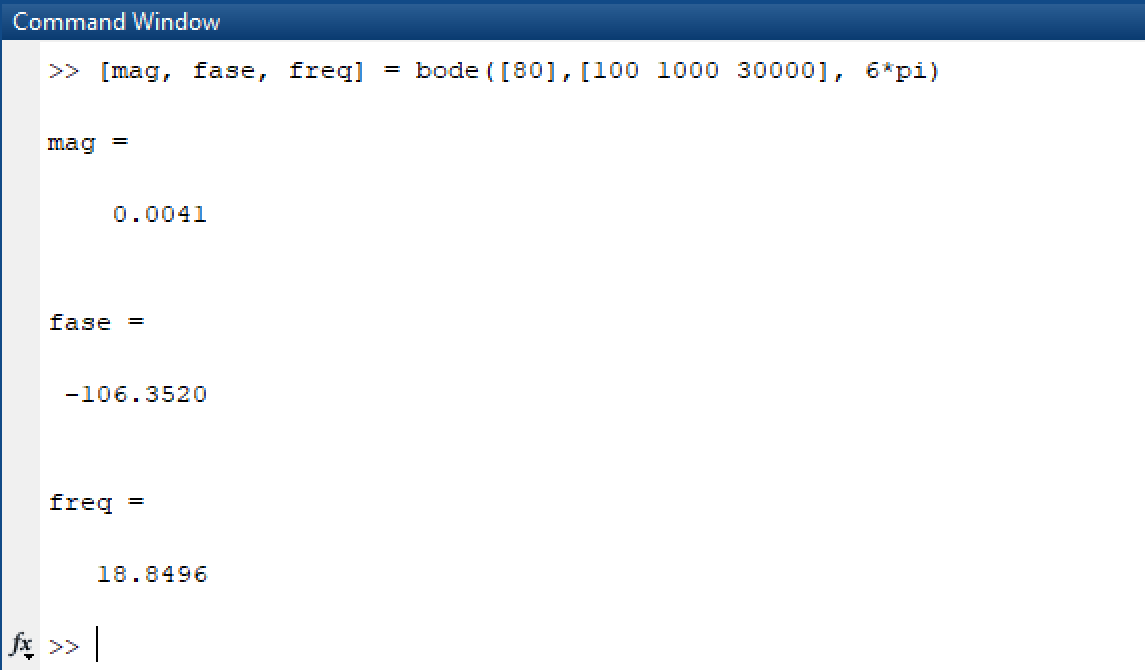
\includegraphics[width=0.85\linewidth]{Figuras/Ch12/fig3.PNG}}
}

\frame{
\frametitle{Exemplo $\#02$ - resposta de regime permanente a uma entrada senoidal}
\begin{block}{}
Uma mola com $K = 857,8$ N/m está fixa em uma extremidade tendo na sua outra extremidade fixado um parafuso de 0,0492 kg, livre para vibrar. A constante de amortecimento do sistema é de 0,11 Kg/s. Determine o coeficiente de amortecimento do sistema. Calcule também a amplitude da resposta de regime permanente quando o sistema é excitado por uma força harmônica de 0,492 N a 125 rad/s. \\
\vspace{0.5cm}
\textbf{Resolução:}
$$M\ddot{x}(t) + B\dot{x}(t) + Kx(t) = F \ sen(\omega t)$$
$$0,0492\ddot{x}(t) + 0,11\dot{x}(t) + 857,8x(t) = 0,492 \ sen(125 t)$$
$$\ddot{x}(t) + 2,2358\dot{x}(t) + 17.434,95x(t) = 10 \ sen(125 t)$$
Na forma padrão, podemos reescrever como sendo:
$$\ddot{x}(t) + 2\zeta\omega_n\dot{x}(t) + \omega_n^2x(t) = f \ sen(\omega t)$$
\end{block}
}

\frame{
\frametitle{Exemplo $\#02$ - resposta de regime permanente a uma entrada senoidal}
\begin{block}{}
Da EDO anterior, temos que:
\begin{itemize}
    \item $\omega_n^2 = 17.434,95 \implies \omega_n \approx 132,04$ rad/s.
    \item $2\zeta\omega_n = 2,2358 \implies \zeta \approx 0,0085$
\end{itemize}
\vspace{0.2cm}
Sendo assim,
$$A = \dfrac{f}{\sqrt{(\omega_n^2 - \omega^2)^2 + (2\zeta\omega_n \omega)^2}} = \dfrac{10}{\sqrt{(17.434,95 - 125^2)^2 + (2,2358 \cdot 125)^2}}$$ \\ $$A \approx 0,00546 \ \text{m.}$$
\end{block}
}

\cprotect\frame{
\frametitle{\MATLAB}
\begin{block}{}
\begin{verbatim}
>>[mag, fase, freq] = bode([num],[den], f)
\end{verbatim}
retorna a resposta na frequência $\bm{f}$ especificada.\\
\end{block}
\centerline{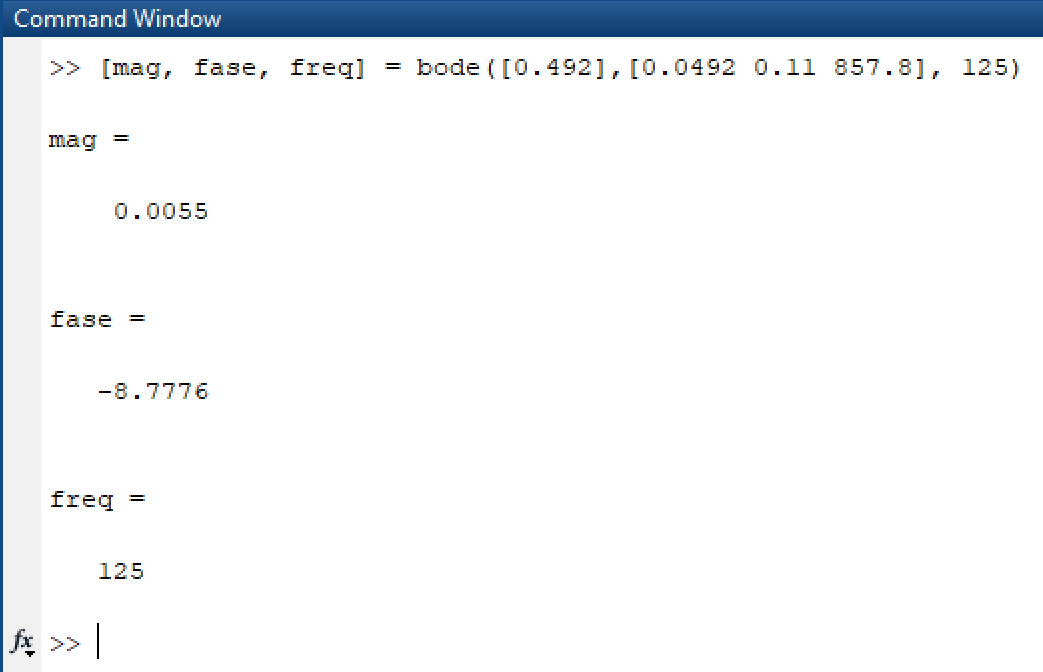
\includegraphics[width=0.8\linewidth]{Figuras/Ch12/fig4.PNG}}
}

\frame{
\frametitle{Resposta de regime permanente a uma entrada senoidal a partir da função de transferência $G(s)$}
\begin{block}{Formulação matemática}
Considere um sistema linear, \textbf{estável} e invariante no tempo.
\begin{itemize}
    \item Entrada: $x(t) = X \ sen(\omega t)$
    \item Saída: $y(t)$
    \item Função de transferência: $G(s) = \dfrac{p(s)}{q(s)} = \dfrac{p(s)}{(s+s_1)(s+s_2) \cdots (s+s_n)}$
\end{itemize}
\end{block}
\centerline{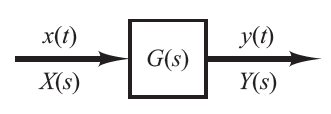
\includegraphics[width=0.5\linewidth]{Figuras/Ch12/fig5.PNG}}
}

\frame{
\frametitle{Resposta de regime permanente a uma entrada senoidal a partir da função de transferência $G(s)$}
\begin{block}{Formulação matemática}
$$Y(s) = G(s)X(s) = G(s)\dfrac{\omega X}{s^2 + \omega^2}$$
$$Y(s) = \dfrac{a}{s+j\omega} + \dfrac{\overline{a}}{s-j\omega} + \dfrac{b_1}{s+s_1} + \dfrac{b_2}{s+s_2} + \cdots + \dfrac{b_n}{s+s_n}$$
onde $a$ e $b_i$ (sendo $i = 1,2,...,n)$ são constantes e $\overline{a}$ é o complexo conjugado de $a$.
$$y(t) = ae^{-j\omega t} + \overline{a}e^{j\omega t} + b_1e^{-s_1 t} + b_2e^{-s_2 t} + ... + b_ne^{-s_n t}$$
\begin{itemize}
    \item Para um sistema estável, conforme $t$ tende a infinito, os termos $e^{-s_1 t}$, $e^{-s_2 t}$, ..., $e^{-s_n t}$ tendem a \textbf{zero}.
    \item Exceto os dois primeiros termos do lado direito da equação se anulam em \textbf{regime permanente}.
\end{itemize}
$$y_{ss}(t) = ae^{-j\omega t} + \overline{a}e^{j\omega t}$$
\end{block}
}

\frame{
\frametitle{Resposta de regime permanente a uma entrada senoidal a partir da função de transferência $G(s)$}
\begin{block}{Formulação matemática}
$$Y(s) = G(s)\dfrac{\omega X}{s^2 + \omega^2} = \dfrac{a}{s+j\omega} + \dfrac{\overline{a}}{s-j\omega}$$
$$a = G(s)\dfrac{\omega X}{s^2 + \omega^2}(s+j\omega)\Big|_{s=-j\omega} = \dfrac{-XG(-j\omega)}{2j}$$
$$\overline{a} = G(s)\dfrac{\omega X}{s^2 + \omega^2}(s-j\omega)\Big|_{s=j\omega} = \dfrac{XG(j\omega)}{2j}$$
\begin{itemize}
    \item Como $G(\pm j\omega)$ é uma grandeza complexa, ela pode ser escrita na forma:
\end{itemize}
$$G(\pm j\omega) = |G(j\omega)|e^{\pm j \phi}$$
onde $|G(j\omega)|$ representa o \textbf{módulo} e $\phi$ representa o \textbf{ângulo}.
\end{block}
}

\frame{
\frametitle{Resposta de regime permanente a uma entrada senoidal a partir da função de transferência $G(s)$}
\begin{block}{Formulação matemática}
Com isso,
$$a = \dfrac{-X|G(j\omega)|e^{-j \phi}}{2j} \qquad \overline{a} = \dfrac{X|G(j\omega)|e^{j \phi}}{2j}$$
Substituindo, obtemos:
$$y_{ss}(t) = \dfrac{-X|G(j\omega)|e^{-j \phi}}{2j}e^{-j\omega t} + \dfrac{X|G(j\omega)|e^{j \phi}}{2j}e^{j\omega t}$$
$$y_{ss}(t) = X|G(j\omega)| \bigg[\dfrac{e^{j
(\omega t + \phi)} - e^{-j
(\omega t + \phi)}}{2j}\bigg]$$
$$y_{ss}(t) = X|G(j\omega)| \ sen(\omega t + \phi)$$
$$y_{ss}(t) = Y \ sen(\omega t + \phi)$$
\end{block}
}

\frame{
\frametitle{Resposta de regime permanente a uma entrada senoidal a partir da função de transferência $G(s)$}
\begin{block}{Conclusões}
\begin{itemize}
    \item $|G(j\omega)| = \bigg|\dfrac{Y(j\omega)}{X(j\omega)}\bigg|$ = relação de \textbf{amplitude}.
    \vspace{0.2cm}
    \item $\phase{G(j\omega)} = \phase{\dfrac{Y(j\omega)}{X(j\omega)}}$ = relação de \textbf{defasagem}.
\end{itemize}
\vspace{0.3cm}
Em consequência, a \textbf{resposta em regime permanente} de um sistema a uma entrada senoidal pode ser obtida diretamente a partir de:
$$G(j\omega) = \dfrac{Y(j\omega)}{X(j\omega)}$$
\begin{itemize}
    \item A função de transferência senoidal de qualquer sistema linear é obtida pela \textbf{substituição} de $s$ por $j\omega$ na função de transferência do sistema.
\end{itemize}
\end{block}
}

\frame{
\frametitle{Exemplo $\#01$ - módulo e fase de uma função de transferência}
\begin{block}{}
Determine $|G(s)|$ e $\phase{G(s)}$, sabendo que $u(t) = sen(2t)$ e 
$$G(s) = \dfrac{10(s+0,5)}{s^2(s+1)(s+2)}$$
\vspace{0.5cm}
\textbf{Resolução:} \\
Como $u(t) = sen(2t)$, temos que $\omega = 2$ rad/s (ponto de teste).
\begin{itemize}
    \item Com o auxílio de um triângulo, marcam-se todos os pontos, do numerador e do denominador.
    \item Avalia-se a \textbf{contribuição individual} de cada ponto.
    \item Na fase, os ângulos do \textbf{denominador} contribuem de forma \textbf{negativa}, ao passo que os ângulos do \textbf{numerador} contribuem de forma \textbf{positiva}.
\end{itemize}
\end{block}
}

\frame{
\frametitle{Exemplo $\#01$ - módulo e fase de uma função de transferência}
\begin{block}{}
$$G(s) = \dfrac{10(s+0,5)}{s^2(s+1)(s+2)}$$
Para o \textbf{módulo}:
\begin{itemize}
    \item $|s+0,5| = \sqrt{2^2 + 0,5^2} = \sqrt{4,25}$
    \item $|s^2| = \sqrt{2^2 + 0^2}^2 = 4$
    \item $|s+1| = \sqrt{2^2 + 1^2} = \sqrt{5}$
    \item $|s+2| = \sqrt{2^2 + 2^2} = \sqrt{8}$
\end{itemize}
Deste modo, $|G(j\omega)| = \dfrac{10 \cdot \sqrt{4,25}}{4 \cdot \sqrt{5} \cdot \sqrt{8}} = 0,8149$
\end{block}
}

\frame{
\frametitle{Exemplo $\#01$ - módulo e fase de uma função de transferência}
\begin{block}{}
$$G(s) = \dfrac{10(s+0,5)}{s^2(s+1)(s+2)}$$
Para a \textbf{fase}:
\begin{itemize}
    \item $\phase{s+0,5} = \text{arctg}(2/0,5) = \SI{75,96}{\degree}$
    \item $\phase{s^2} = 2 \cdot \SI{90}{\degree} = \SI{180}{\degree}$
    \item $\phase{s+1} = \text{arctg}(2/1) = \SI{63,43}{\degree}$
    \item $\phase{s+2} = \text{arctg}(2/2) = \SI{45}{\degree}$
\end{itemize}
Deste modo, $\phase{G(j\omega)} = \SI{75,96}{\degree} - \SI{180}{\degree} - \SI{63,43}{\degree} - \SI{45}{\degree} = \SI{-212,47}{\degree}$
\end{block}
}

\frame{
\frametitle{Exemplo $\#02$ - módulo e fase de uma função de transferência}
\begin{block}{Problema}
Obtenha a amplitude e fase da resposta em regime permanente para o circuito elétrico abaixo quando $i_i(t) = sen(t)$.
\end{block}
\centerline{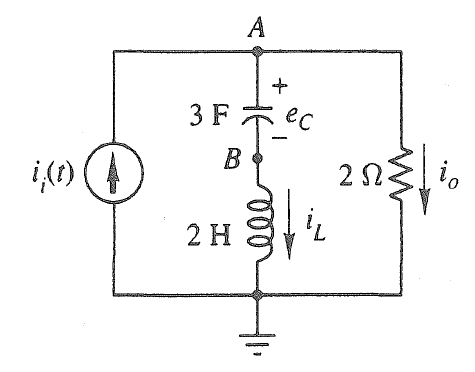
\includegraphics[width=0.5\linewidth]{Figuras/Ch12/fig6.PNG}}
}

\frame{
\frametitle{Exemplo $\#02$ - módulo e fase de uma função de transferência}
\begin{block}{Resolução}
\begin{itemize}
    \item Análise no \textbf{nó $\bm{A}$}: $3 (\dot{e}_A - \dot{e}_B) + \dfrac{1}{2}e_A = i_i(t)$
    \vspace{0.2cm}
    \item Análise no \textbf{nó $\bm{B}$}: $i_L(0) + \dfrac{1}{2}{\displaystyle \int_{0}^{t}} e_B(\lambda) d\lambda = 3 (\dot{e}_A - \dot{e}_B)$
    \vspace{0.2cm}
    \item A \textbf{saída} é dada como: $i_0 = \dfrac{1}{2}e_A$
\end{itemize}
Considerando as condições iniciais nulas, as transformadas de Laplace são:
\begin{equation*}
    \begin{cases}
    \Big(3s + \dfrac{1}{2}\Big)E_A(s) - 3sE_B(s) = I_i(s) \\
    -3sE_A(s) + \Big(3s + \dfrac{1}{2s}\Big)E_B(s) = 0 \\
    I_0(s) = \dfrac{1}{2}E_A(s)
    \end{cases}
\end{equation*}
\end{block}
}

\frame{
\frametitle{Exemplo $\#02$ - módulo e fase de uma função de transferência}
\begin{block}{Resolução}
Manipulando as equações e isolando para $I_0(s)$ e $I_i(s)$, chega-se em:
$$H(s) = \dfrac{I_0(s)}{I_i(s)} = \dfrac{6s^2 + 1}{6s^2 + 6s + 1} \implies H(j\omega) = \dfrac{6(j\omega)^2 + 1}{6(j\omega)^2 + 6(j\omega) + 1}$$
Deste modo, $|H(j\omega)|\big|_{\omega=1} = \Bigg|\dfrac{-6+1}{-6+6j+1}\Bigg| = \dfrac{\sqrt{(-5)^2}}{\sqrt{6^2 + (-5)^2}} = 0,64$ \\
\vspace{0.2cm}
Além disso, $\phase{H(j\omega)}\big|_{\omega=1} = \phase{\dfrac{-5}{6j-5}} = \text{arctg}(0) - \text{arctg}(6/-5) = 0,876 \ \text{rad}$
\vspace{0.2cm}
\end{block}
}

\frame{
\frametitle{Exercícios}
\begin{block}{}
01. Considere um sistema massa-mola-amortecedor com duas molas $K_1$ e $K_2$ conectadas em série, montado em um carro de massa desprezível. Determine a amplitude e a fase da resposta de regime permanente de $x$ quando este sofre uma oscilação $u$ de 0,2 m de amplitude a uma frequência de 2 rad/s. Sabe-se que $K_1 = K_2 = 2$ N/m, $B = 1$ Ns/m e $M = 0,25$ Kg. Despreze qualquer atrito, exceto aquele produzido pelo dispositivo amortecedor. 

\vspace{0.5cm}

02. Calcule a amplitude e fase da resposta de regime permanente do sistema descrito no exercício anterior a partir de sua função de transferência.
\end{block}
}

\frame{
\frametitle{Referências e exercícios complementares}
\begin{itemize}
\item NISE, Norman S. Engenharia de Sistemas de Controle, 7 ed. LTC, 2017.
\end{itemize}
\centering{\alert{Página 499 - \textbf{Capítulo 10}}} \\
\vspace{0.4cm}
\begin{itemize}
\item OGATA, Katsuhiko. Engenharia de Controle Moderno, 5 ed. Pearson, 2010.
\end{itemize}
\centering{\alert{Página 513 - \textbf{Capítulo 7}}} \\
}